\documentclass[border=15pt, tikz]{standalone}
\usepackage[T1]{fontenc}
\usepackage[utf8]{inputenc}
\usepackage{tikz}
\usetikzlibrary{positioning, arrows.meta, decorations.pathreplacing, calc, fit}
\definecolor{clrattention}{HTML}{6B9BD2}
\definecolor{clrattention_alt}{HTML}{A8C8E8}
\definecolor{clrffn}{HTML}{D4956A}
\definecolor{clrnorm}{HTML}{E8D78E}
\definecolor{clrembed}{HTML}{7DB892}
\definecolor{clrresidual}{HTML}{8EAEC8}
\definecolor{clroutput}{HTML}{B08EAF}
\definecolor{clrspectral}{HTML}{7BC8C8}
\definecolor{clrphysics}{HTML}{D4956A}
\definecolor{clrborder}{HTML}{4A4A4A}
\definecolor{clrtext}{HTML}{333333}
\definecolor{clrgroup_frame}{HTML}{AAAAAA}
\definecolor{clrgroup_fill}{HTML}{F5F5F5}
\begin{document}
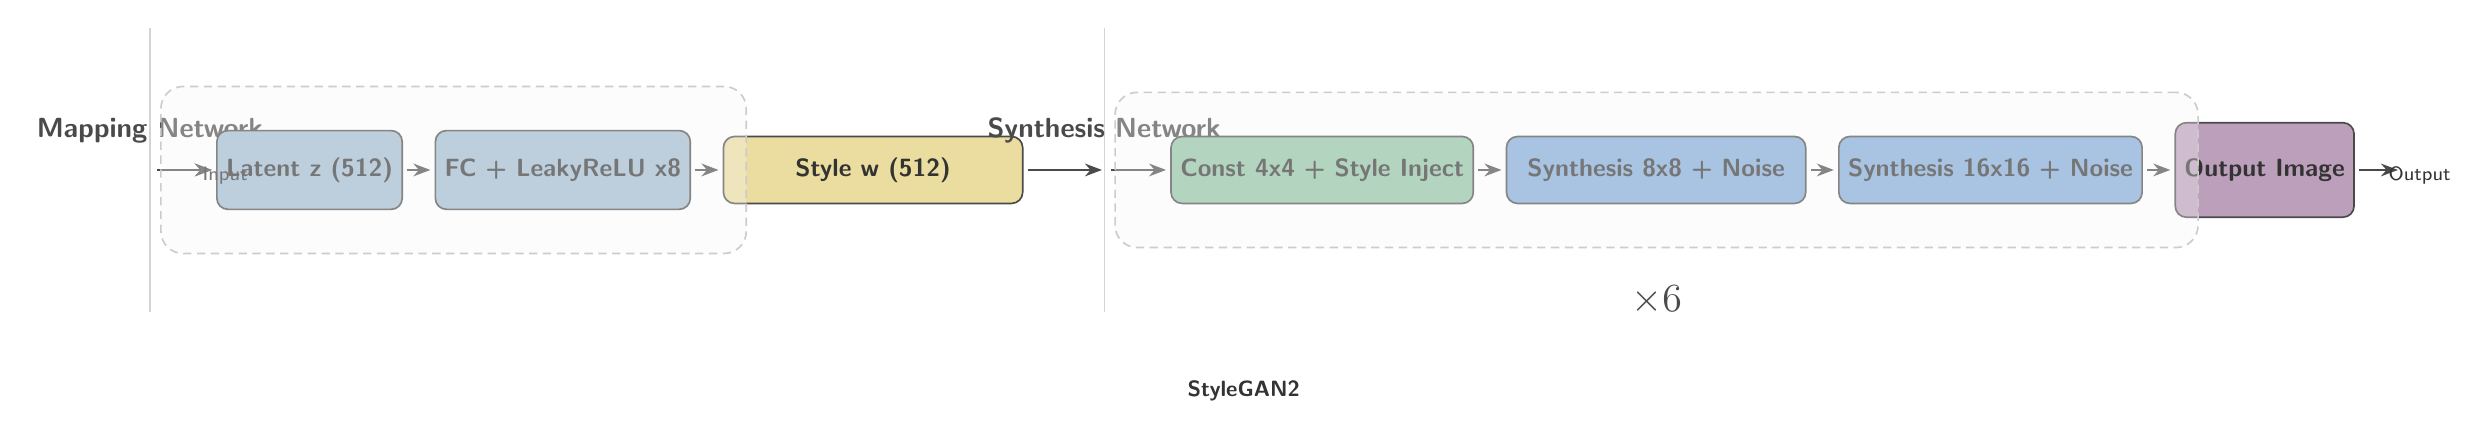
\begin{tikzpicture}[
    >=Stealth,
    every node/.style={font=\sffamily},
    block/.style={draw=clrborder, rounded corners=4pt, minimum width=3.8cm,
                  minimum height=0.85cm, font=\sffamily\small\bfseries,
                  text=clrtext, line width=0.6pt},
    arrow/.style={->, thick, color=clrborder, line width=0.7pt, shorten >=1.5pt, shorten <=1.5pt},
    skiparrow/.style={->, thick, color=clrresidual, line width=0.8pt, rounded corners=4pt, shorten >=1.5pt},
    label/.style={font=\sffamily\scriptsize, text=clrtext},
    subtitle/.style={font=\sffamily\footnotesize, text=clrtext},
]
\node[inner sep=0, minimum height=0] (n_1_rule) at (0,0) {};
\draw[color=clrgroup_frame!50, line width=0.4pt] ([yshift=-1.8cm]n_1_rule.center) -- ([yshift=1.8cm]n_1_rule.center);
\node[right=0pt of n_1_rule, inner sep=0, minimum size=0] (n_1) {};
\node[above=6pt of n_1_rule, font=\sffamily\normalsize\bfseries, text=clrborder] (n_1_title) {Mapping Network};
\node[block, fill=clrresidual!85, minimum width=2.0cm, minimum height=1.0cm, text=clrtext, right=0.8cm of n_1] (n_2) {Latent z (512)};
\node[block, fill=clrresidual!85, minimum width=2.0cm, minimum height=1.0cm, text=clrtext, right=0.4cm of n_2] (n_3) {FC + LeakyReLU x8};
\node[block, fill=clrnorm!85, minimum width=3.8cm, minimum height=0.85cm, text=clrtext, right=0.4cm of n_3] (n_4) {Style w (512)};
\node[inner sep=0, minimum height=0, right=1.0cm of n_4] (n_5_rule) {};
\draw[color=clrgroup_frame!50, line width=0.4pt] ([yshift=-1.8cm]n_5_rule.center) -- ([yshift=1.8cm]n_5_rule.center);
\node[right=0pt of n_5_rule, inner sep=0, minimum size=0] (n_5) {};
\node[above=6pt of n_5_rule, font=\sffamily\normalsize\bfseries, text=clrborder] (n_5_title) {Synthesis Network};
\node[block, fill=clrembed!85, minimum width=3.8cm, minimum height=0.85cm, text=clrtext, right=0.8cm of n_5] (n_6) {Const 4x4 + Style Inject};
\node[block, fill=clrattention!85, minimum width=3.8cm, minimum height=0.85cm, text=clrtext, right=0.4cm of n_6] (n_7) {Synthesis 8x8 + Noise};
\node[block, fill=clrattention!85, minimum width=3.8cm, minimum height=0.85cm, text=clrtext, right=0.4cm of n_7] (n_8) {Synthesis 16x16 + Noise};
\node[block, fill=clroutput!85, minimum width=2.0cm, minimum height=1.2cm, text=clrtext, right=0.4cm of n_8] (n_9) {Output Image};
\draw[arrow] (n_1.east) -- (n_2.west);
\draw[arrow] (n_2.east) -- (n_3.west);
\draw[arrow] (n_3.east) -- (n_4.west);
\draw[arrow] (n_4.east) -- (n_5.west);
\draw[arrow] (n_5.east) -- (n_6.west);
\draw[arrow] (n_6.east) -- (n_7.west);
\draw[arrow] (n_7.east) -- (n_8.west);
\draw[arrow] (n_8.east) -- (n_9.west);
\draw[arrow] ([xshift=-0.6cm]n_2.west) -- node[right, yshift=-2pt, font=\sffamily\scriptsize, text=clrtext] {Input} (n_2.west);
\draw[arrow] (n_9.east) -- node[right, yshift=-2pt, font=\sffamily\scriptsize, text=clrtext] {Output} ([xshift=0.6cm]n_9.east);
\node[draw=clrgroup_frame!60, rounded corners=8pt, densely dashed, line width=0.6pt, fill=clrgroup_fill, fill opacity=0.35, inner ysep=0.55cm, inner xsep=0.7cm, fit=(n_2) (n_3)] (g_0) {};
\node[draw=clrgroup_frame!60, rounded corners=8pt, densely dashed, line width=0.6pt, fill=clrgroup_fill, fill opacity=0.35, inner ysep=0.55cm, inner xsep=0.7cm, fit=(n_6) (n_7) (n_8)] (g_1) {};
\node[below=10pt of g_1.south, anchor=north, font=\sffamily\Large\bfseries, text=clrborder] (g_1_badge) {$\times6$};
\node[below=0.6cm of current bounding box.south, subtitle, text width=14cm, align=center] {\textbf{StyleGAN2}};
\end{tikzpicture}
\end{document}
